% !TEX root = ../Thesis.tex
\newcommand{\Wplus}{\ensuremath{W^{+}}}
\newcommand{\Wminus}{\ensuremath{W^{\minus}}}

\chapter[Measurement of the \ttbar\ cross-section]{Measurement of the \ttbar\ cross-section in the $\ell$+jets channel using SMT} \label{ch:CrossSection}

\textit{This section describes a \ttbar\ cross-section measurement carried out the joint RHUL-QMUL SMT group.}

Measurement of the \ttbar\ production cross-section is important for two reasons. First, the value of the \ttbar\ cross-section is a powerful test of the SM and perturbative QCD. Additionally, \ttbar\ events constitute a background to other analyses such as SUSY searches and Higgs boson searches and properties studies. Presented here is a measurement of the top-pair production cross-section at \cmsS\ in the lepton plus jets channel, with at least one of the $b$-quarks in the event decaying semileptonically producing a soft muon. The presence of such a jet is determined by the use of the \xsm-based SMT tagger.

\section{The SMT Tagger} \label{sec:SMTExplanation}
The SMT tagger which forms the focus of this thesis is based on the \xsm\ of the STACO combined muon as described in Section~\ref{sec:DetectorSTACO}. The SMT tagger associates good quality jets with SMT candidate muons, a selection is then applied to the muons based around the \xsm\ from the STACO combination.

The SMT candidates are required to lie within the coverage of the ID ($|\eta|<2.5$) and have a sufficiently high \pt\ for reliable muon reconstruction (\pt>\SI{4}{\GeV}). In addition, requirements are made on the impact parameters of the muon $|d_{0}|<$\SI{3}{\mm} and $|z_{0}\sin{\theta}|<$\SI{3}{\mm}, to reduce contributions from the decay of long-lived hadrons ($\pi$ and $K$), interactions with the beam pipe material and pile-up at high luminosity.

\section{Data and Monte Carlo samples} \label{sec:CrossSectionSamplesMC}

\section{Object selection and event selection} \label{sec:CrossSectionEventSelection}
The selection criteria used in this analysis are based on the nominal \cmsS\ selections constructed by the ATLAS top group. Some alterations have been implemented to adapt to the usage of the \xsm-tagger instead of the standard MV1 method for $b$-jet tagging. 

\section{Background estimation} \label{sec:CrossSectionBacgkround}

Semi-leptonic \ttbar\ events have a varied final state signature that includes a lepton, multiple jets including $b$-jets and missing energy. As a result \ttbar\ analyses must take into account many different types of background including diboson, \W+jets, \Z+jets, single-top and multijet. Data-driven methods are used for the dominant multijet and \W+jets backgrounds while MC is used to estimate the smaller \Z+jets, diboson and single-top.

\subsection{Multijet in the electron channel}
The multijet background is a difficult background to reduce and estimate. Measurement of multijet events depends very strongly on detector conditions, which in turn depend on external factors which cannot be simulated. Multijet events that pass the event selection include non-isolated or misidentified electrons from photon conversion or charged hadrons. As a result, data-driven methods must be employed when estimating the amount of multijet background. This analysis makes use of two different methodologies, The so-called matrix method is used for the central value of the estimate and the ABCD method for verification and use as a systematic.

At pretag level the multijet content in the signal region is estimated by using the matrix method. In addition to the standard electron selection a looser selection is defined. Events are categorized by whether they pass the loose or standard selection. The number of events in each category is the sum of events with ``real'' electrons and ``fake'' electrons as follows:
%
\begin{align*}
  N^{\textrm{loose}} &= N_{\textrm{real}}^{\textrm{loose}} + N_{\textrm{fake}}^{\textrm{loose}} \\
  %
  N^{\textrm{std}} &= rN_{\textrm{real}}^{\textrm{loose}} + fN_{\textrm{fake}}^{\textrm{loose}}
\end{align*}
%
where $r$ and $f$ are the ``real'' and ``fake'' efficiencies for the loose event to also pass the standard selection. Given a measured $N^{\textrm{std}}$ and $N^{\textrm{loose}}$ and if $f$ and $r$ are known the number of events with a fake electron that passes the standard selection can be calculated as
%
\begin{equation*}
  N_{\textrm{fake}}^{\textrm{std}} = fN_{\textrm{fake}}^{\textrm{loose}} = f\frac{N^{\textrm{std}}-r N^{\textrm{loose}} }{(f-r)}
\end{equation*}

The relative efficiency $r$ is measured from an inclusive sample of $Z\rightarrow ee$ events and $f$ is measured from a sample of events with exactly one loose electron, at least one jet with a \pt$>$\SI{25}{\GeV} and \met$<${20}{\GeV}. An uncertainty of $50\%$ is assigned to the pretag estimate to cover the respective uncertainties on $f$ and $r$.

To derive the tagged estimate the pretag estimates are scaled by the probability of SMT tagging an event. The tagging probability of multijet events $R_{\textrm{SMT}}^{\textrm{multijet}}$ is derived from control regions defined by the isolation of the electron and the \met\ cut that forms part of the event selection, as shown in Figure~\ref{fig:CrossSectionABCDRegions}.

\begin{figure}[htbp]
  \centering
  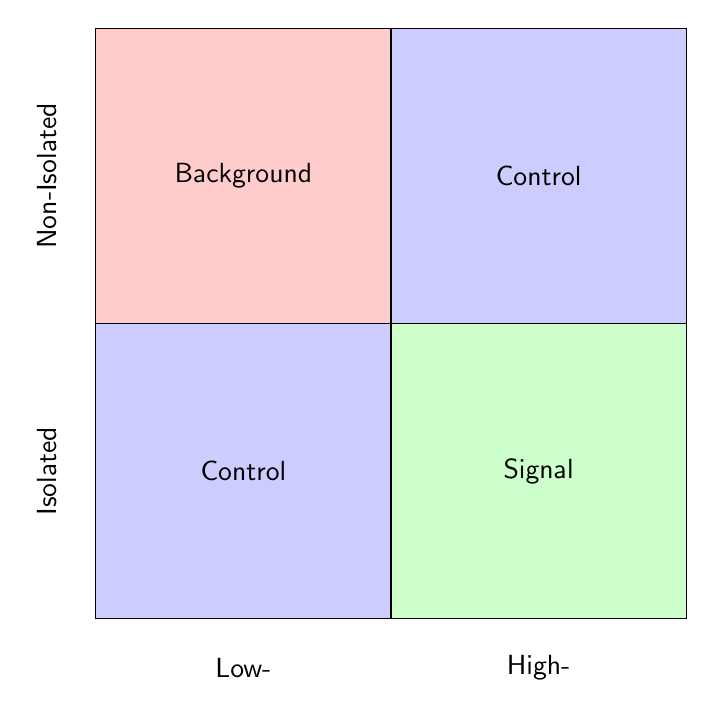
\begin{tikzpicture}[font=\sffamily]
  \tikzstyle{region}=[draw=black, minimum height=3.75cm,minimum width=3.75cm, fill=yellow!20, node distance=3.75cm]
  \tikzstyle{Signal}=[region, fill=green!20]
  \tikzstyle{Bkg}=[region, fill=red!20]
  \tikzstyle{Control}=[region, fill=blue!20]
  \tikzstyle{xLabel} = [font={\sffamily}, minimum width=3.75cm, node distance=3.75cm,node distance=2.5cm]
  \node[name=bkgregion, Bkg]{Background};
  \node[name=notIsolated, left of = bkgregion, xLabel, rotate=90] {Non-Isolated};
  \node[name=control1, right of = bkgregion, Control] {Control};

  \node[name=control2, below of = bkgregion, Control] {Control};
  \node[name=Isolated, left of = control2, xLabel, rotate=90] {Isolated};
  \node[name=signal, right of = control2, Signal] {Signal};
  \node[name=highMetLabel, xLabel, below of = signal] {High-\met};
  \node[name=lowMetLabel, xLabel, below of = control2] {Low-\met};
  \end{tikzpicture}  
  \caption{A diagram of the \met-isolation phase space. Shown are the four regions as defined by the event selection.}
  \label{fig:CrossSectionABCDRegions}
\end{figure}

These four regions can be identified as a background-dominated region, containing events with low-\met\ and a non-isolated electron; a signal region, with events that pass the event selection; and two control regions, containing events with high-\met\ or an isolated electron. The events in each of the regions then represents a different type of phenomenon. The tagging rate is simply defined as
%
\begin{equation*}
  R_{\textrm{SMT}} = \frac{N_{Tagged}}{N_{Pretag}} 
\end{equation*}
%
where $N$ is the number of events in the region. Contributions from other processes such as $W$+jets, $Z$+jets, \ttbar, single-top and diboson events are subtracted using MC simulation. Thus the yield in each region is defined as
%
\begin{equation*}
  N^{\textrm{multijet}} = N^{\textrm{data}} - N^{W+\textrm{jets}} - N^{Z+\textrm{jets}} - N^{\textrm{diboson}} - N^{\ttbar} - N^{\textrm{single-top}}
\end{equation*}

The contribution from \ttbar\ is initially based on the theoretical cross-section, an estimate for the multijet contribution is determined using this cross-section and a new measured cross-section is obtained. The measured cross-section is used to rescale the \ttbar\ contribution and a new cross-section is obtained. This process is repeated until the measured cross-section stablizes after two iterations.

The uncertainty on the tagging-rate contains statistical and a systematic contributions. The systematic uncertainty includes the uncertainty on the cross-section of the \ttbar\ and $W$+jets samples, uncertainty arising from the SMT tagger and finally uncertainties arising from the BR re-weighting described a priori.

The final tagging-rate is the unweighted average of all the regions. The uncertainty is the difference between regions A and C, as this is larger than any regional uncertainty. The tagging-rate and subsequently the tagged multijet background estimate is measured on a per-jet bin basis. The tagging-rates per region for each jet-bin are shown in Table~\ref{tab:rsmt}.

\begin{table}[htbp]
  \centering
    \begin{tabular}{r|cccc}
      \hline
      Jet-bin & $R^{\textrm{SMT}}_{\textrm{A}}$ & $R^{\textrm{SMT}}_{\textrm{B}}$ & $R^{\textrm{SMT}}_{\textrm{C}}$ & $R^{\textrm{SMT}}_{\textrm{A}VG}$ \\ \hline \hline
      1      & 0.91$\pm$0.03 & 0.82$\pm$0.10 & 0.51$\pm$0.05 & 0.64$\pm$0.07 \\
      2      & 1.8$\pm$0.1   & 2.0$\pm$0.2   & 1.3$\pm$0.1   & 1.5$\pm$0.1 \\
      3      & 2.8$\pm$0.1   & 2.5$\pm$1.1   & 2.5$\pm$0.5   & 2.6$\pm$1.0 \\
      $\ge$3 & 3.84$\pm$0.09 & 3.7$\pm$1.3   & 3.0$\pm$0.8   & 3.2$\pm$1.2 \\
      $\ge$4 & 3.2$\pm$0.1   & 3.7$\pm$1.3   & 3.0$\pm$0.8   & 3.2$\pm$1.2 \\
      \hline
    \end{tabular}
    \caption{Multijet SMT event taggin-rate(in percent) in regions A) inverted-\met, non-isolated, B) High-\met, non-isolated and C) low-\met, isolated.} \label{tab:rsmt}
\end{table}

\begin{table}[!htbp]
    \centering
    \begin{tabular}{r|cc}
      \hline % ----------------------------
      Jet-bin & Pretag          & Tagged \\
      \hline % ----------------------------
      1       & 51000$\pm$26000 & 330$\pm$160 \\ 
      2       & 26000$\pm$13000 & 400$\pm$200 \\
      3       & 8100$\pm$4100   & 210$\pm$130 \\ 
      $\ge$3  & 10800$\pm$5400  & 330$\pm$210 \\ 
      \hline % ----------------------------
    \end{tabular}
    \caption{Multijet estimates in the e+jets obtained by the jet-electron method. The uncertainties are combined statistical and systematics. A systematic uncertainty of 50\% is used on the jet-electron pretag event yields~\cite{TopQuark:SingleXSectionTChannel} in addition to e uncertainties obtained on $R^{\textrm{SMT}}_{\textrm{WGT}}$.} \label{tab:rsmtest}
  \end{table}

\subsubsection{The ABCD method}
The ABCD method relies on a pair of uncorrelated variables to extrapolate the amount of multijet events from a set of control regions into the signal region. First a two-dimensional phase-space is constructed, in this case the same two variables, missing energy and isolation are used. If these two variables are uncorrelated then the following relation holds
%
\begin{equation}
  N^{\textrm{multijet}}_{\textrm{D}} = \frac{N^{\textrm{multijet}}_{\textrm{B}} * N^{\textrm{multijet}}_{\textrm{C}}}{N^{\textrm{multijet}}_\textrm{A}}
\end{equation} 
%
where $N^{\textrm{multijet}}_{X}$ is the number of multijet events in region $\textrm{X}$.

This allows for an estimation of the number of multijet events that pass the event selection by extrapolating from the background region into the signal region. As with the matrix method, event contributions from other processes are removed using MC. The uncertainty on the final estimate includes statistical contributions from the yield in each region and the systematinc uncertainty on the $W$+jets and \ttbar\ samples as described.

\subsection{Multijet background in the muon channel}
Multijet events contaimnate the signal region by producing ``fake'' isolated muons which are misidentified as signal muons. The main sources of fake muons are semileptonic decay of heavy quarks ($b$/$c$), muons from the decay in flight of pions and kaons and ``punch-through'' of hadrons not fully absorbed by the hadronic calorimeter and produce a signal in the muon system.

The procedure in the muon channel is similar to that used for the electron channel. A pretag estimate of the multijet fraction in the signal region is obtained using the matrix method. The ``real'' muon selection efficiency $r$ is measured from an inclusive sample of $Z\rightarrow\mu\mu$ events. The ``fake'' muon selection efficiency $f$ is obtained from data using two different methods:

\begin{itemize}
  \item a control region where the $\met+\mtw$ cut is inverted and an additional cut of $\mtw<$\SI{20}{\GeV} is applied,
  \item and a fit to the transverse impact parameter significance $\sigma_{d_{0}}$ distribution where both $\met+\mtw$ and $\met$ cuts are inverted.
\end{itemize}

The central value of the pretag estimate is obtained from an average of these two regions. An uncertainty of \SI{20}{\percent} is assigned to the final estimate to account for the uncertainty associated with each region and the difference between them.

The SMT event tagging rate is obtained from two control regions, defined by inverting the \met\ and $\met+\mtw$ cuts, and by inverting the muon isolation requirement.
Finally, the sources of uncertainty are the same as those considered in the electron channel.

\subsection{$W$+jets background}

The $W$+jets background is the most dominant background since these events contain a real lepton and \met\ from the escaping neutrino. Events can be classified into $W$+HF, which is the largest contribution; and $W$+LF where a LF jet is mis-tagged. Due to the significant uncertainty on the overall normalization of $W$+jets and the presence of a mis-tagged LF jet, a data-driven method, known as $W$ charge asymmetry~\cite{Measurement}, is used to estimate this background.

The $W$ charge asymmetry method relies on the observation that the ratio of positive to negative $W$ bosons suffers from small theoretical uncertainty and thus can provide an overall normalization. Thus the overall normalization is by
%
\begin{equation}
  \begin{aligned}
  N_{W^{+}}+N_{W^{-}} &= \frac{N^{\textrm{MC}}_{W^{+}} + N^{\textrm{MC}}_{W^{-}} }{ N^{\textrm{MC}}_{W^{+}} - N^{\textrm{MC}}_{W^{-}} } (D^{+} - D^{-}) \\
                      &= \frac{r_{\textrm{MC}} + 1}{r_{\textrm{MC}} - 1} (D^{+} - D^{-})
  \end{aligned}
\end{equation}
%
where $r_{\textrm{MC}}$ is the ratio in MC of events with a positive lepton to those with a negative lepton and $D^{\pm}$ are the number of events in data with a positive or negative lepton. Contributions from other charge asymmetric processes, namely single-top and diboson are removed using MC simulation. This results in an overall normalization for the $W$+jets background at the pretag level. For the tagged level an event tagging rate is obtained for the $W$+HF and $W$+LF components separately:
%
\begin{equation*}
  W_{\textrm{tag}} = R^{\textrm{LF}}_{\textrm{tag}}W^{\textrm{LF}}_{\textrm{pretag}} + \sum_{\textrm{HF}}^{\textrm{HF}=c,cc,bb} R^{\textrm{HF}}_{\textrm{tag}}W^{\textrm{HF}}_{\textrm{pretag}}
\end{equation*}
% 
where $R^{\textrm{LF}}_{\textrm{tag}}$ is defined as the probability to mistag a LF event and $R^{\textrm{HF}}_{\textrm{tag}}$ is the probability to correctly tag a HF event. The tagging rates are obtained from simulation with the SMT scale factors and BR reweighting applied to each tagged jet.

\section{Systematic uncertainties} \label{sec:systematics_uncertainties}

\section{Results and conclusion} \label{sec:results_and_conclusion}

The final cross-section is determined by a cut-and-count method. Finally the cross-section is calcuated as

\begin{equation}
  \sigma_{\ttbar} = \frac{N_{\textrm{data}} - N_{\textrm{bkg}}}{\int L \textrm{ d}t \times \epsilon \times \textrm{BR(noFullHad)}}
\end{equation}

The cross-section measured in the electron
%


